\subsection{Задание 4}%
\label{subsec:4}%
a=6.1, b=9.46\newline%
\newline%
%
Исходные данные неупорядоченные:\newline%
\newline%
%
\begin{changemargin}{-4cm}{0cm}\small{%
\begin{tabular}{|p{0.08\linewidth}|p{0.08\linewidth}|p{0.08\linewidth}|p{0.08\linewidth}|p{0.08\linewidth}|p{0.08\linewidth}|p{0.08\linewidth}|p{0.08\linewidth}|p{0.08\linewidth}|p{0.08\linewidth}|}%
\hline%
8.91018&8.29374&8.88958&7.82780&7.18405&8.26589&6.21151&7.97928&7.34325&6.36996\\%
\hline%
9.11988&6.41875&8.54347&7.53926&7.47544&8.74177&7.98634&8.79624&7.42303&6.72877\\%
\hline%
8.34361&8.41191&9.30401&9.11602&7.72913&6.93243&7.18277&7.87913&8.84123&6.11534\\%
\hline%
7.96888&6.52646&8.84283&6.84004&8.03695&6.29181&7.66479&8.03671&9.03393&7.78612\\%
\hline%
8.13577&7.26322&8.34620&6.59104&6.69418&6.85422&7.27710&7.80982&9.03941&6.12182\\%
\hline%
8.29152&8.41330&8.28312&7.62500&9.14764&7.25201&9.33478&7.89168&8.23778&6.64248\\%
\hline%
7.25703&7.85996&6.45092&8.63611&9.06575&9.45048&6.89406&8.23378&8.94944&8.28389\\%
\hline%
6.55950&6.14309&7.95383&7.79261&9.32830&6.16251&6.28815&6.15730&6.63312&8.06298\\%
\hline%
6.70774&7.18827&8.97618&8.09306&8.43732&8.96131&9.35969&6.40913&6.59176&9.42594\\%
\hline%
9.03436&7.04502&9.01711&6.73079&6.99592&8.32178&6.38252&8.40200&8.99550&7.72097\\%
\hline%
6.56796&9.28245&7.59856&8.26254&7.71560&6.45940&6.94121&6.73281&8.69295&6.61194\\%
\hline%
8.20903&7.65358&9.34045&8.08651&8.68740&8.79739&8.91552&8.86526&6.23377&6.80823\\%
\hline%
9.43452&8.78930&7.72378&8.82037&8.66729&6.49833&7.50621&9.39192&7.25589&8.61802\\%
\hline%
7.49210&8.48937&7.66874&8.90013&8.12496&7.06294&8.11783&7.22483&6.87096&8.51242\\%
\hline%
6.87425&7.98371&7.20591&9.02850&7.32478&6.18167&8.02286&8.56844&7.95505&8.42831\\%
\hline%
8.87303&6.44637&7.42033&8.22613&6.71621&8.45465&8.06748&8.12885&9.31020&7.26715\\%
\hline%
9.10767&7.31474&7.27326&9.12497&9.34991&9.01500&8.83140&6.16709&8.93067&6.70706\\%
\hline%
6.56325&9.08311&7.81939&8.71664&7.91669&8.07958&6.58481&9.07679&8.56668&9.28042\\%
\hline%
8.89296&8.66596&7.11508&6.64348&8.55324&9.03839&8.06943&8.37293&7.16686&7.92852\\%
\hline%
8.31200&6.47938&9.06770&9.04886&8.86859&7.81672&6.24946&8.15619&9.27625&8.15770\\%
\hline%
\end{tabular}%
\newline%
\newline%
%
}\end{changemargin}%
\newpage%
Исходные данные упорядоченные:\newline%
\newline%
%
\begin{changemargin}{-4cm}{0cm}\small{%
\begin{tabular}{|p{0.08\linewidth}|p{0.08\linewidth}|p{0.08\linewidth}|p{0.08\linewidth}|p{0.08\linewidth}|p{0.08\linewidth}|p{0.08\linewidth}|p{0.08\linewidth}|p{0.08\linewidth}|p{0.08\linewidth}|}%
\hline%
6.11534&6.12182&6.14309&6.15730&6.16251&6.16709&6.18167&6.21151&6.23377&6.24946\\%
\hline%
6.28815&6.29181&6.36996&6.38252&6.40913&6.41875&6.44637&6.45092&6.45940&6.47938\\%
\hline%
6.49833&6.52646&6.55950&6.56325&6.56796&6.58481&6.59104&6.59176&6.61194&6.63312\\%
\hline%
6.64248&6.64348&6.69418&6.70706&6.70774&6.71621&6.72877&6.73079&6.73281&6.80823\\%
\hline%
6.84004&6.85422&6.87096&6.87425&6.89406&6.93243&6.94121&6.99592&7.04502&7.06294\\%
\hline%
7.11508&7.16686&7.18277&7.18405&7.18827&7.20591&7.22483&7.25201&7.25589&7.25703\\%
\hline%
7.26322&7.26715&7.27326&7.27710&7.31474&7.32478&7.34325&7.42033&7.42303&7.47544\\%
\hline%
7.49210&7.50621&7.53926&7.59856&7.62500&7.65358&7.66479&7.66874&7.71560&7.72097\\%
\hline%
7.72378&7.72913&7.78612&7.79261&7.80982&7.81672&7.81939&7.82780&7.85996&7.87913\\%
\hline%
7.89168&7.91669&7.92852&7.95383&7.95505&7.96888&7.97928&7.98371&7.98634&8.02286\\%
\hline%
8.03671&8.03695&8.06298&8.06748&8.06943&8.07958&8.08651&8.09306&8.11783&8.12496\\%
\hline%
8.12885&8.13577&8.15619&8.15770&8.20903&8.22613&8.23378&8.23778&8.26254&8.26589\\%
\hline%
8.28312&8.28389&8.29152&8.29374&8.31200&8.32178&8.34361&8.34620&8.37293&8.40200\\%
\hline%
8.41191&8.41330&8.42831&8.43732&8.45465&8.48937&8.51242&8.54347&8.55324&8.56668\\%
\hline%
8.56844&8.61802&8.63611&8.66596&8.66729&8.68740&8.69295&8.71664&8.74177&8.78930\\%
\hline%
8.79624&8.79739&8.82037&8.83140&8.84123&8.84283&8.86526&8.86859&8.87303&8.88958\\%
\hline%
8.89296&8.90013&8.91018&8.91552&8.93067&8.94944&8.96131&8.97618&8.99550&9.01500\\%
\hline%
9.01711&9.02850&9.03393&9.03436&9.03839&9.03941&9.04886&9.06575&9.06770&9.07679\\%
\hline%
9.08311&9.10767&9.11602&9.11988&9.12497&9.14764&9.27625&9.28042&9.28245&9.30401\\%
\hline%
9.31020&9.32830&9.33478&9.34045&9.34991&9.35969&9.39192&9.42594&9.43452&9.45048\\%
\hline%
\end{tabular}%
\newline%
\newline%
%
}\end{changemargin}%
\newpage%
Интервальный ряд:\newline%
\newline%
%
\begin{tabular}{|c|c|c|}%
\hline%
Интервалы&$n_i$&$w_i$\\%
\hline%
{[}6.10000,6.52000{]}&21.00000&0.10500\\%
\hline%
{[}6.52000,6.94000{]}&25.00000&0.12500\\%
\hline%
{[}6.94000,7.36000{]}&21.00000&0.10500\\%
\hline%
{[}7.36000,7.78000{]}&15.00000&0.07500\\%
\hline%
{[}7.78000,8.20000{]}&32.00000&0.16000\\%
\hline%
{[}8.20000,8.62000{]}&28.00000&0.14000\\%
\hline%
{[}8.62000,9.04000{]}&34.00000&0.17000\\%
\hline%
{[}9.04000,9.46000{]}&24.00000&0.12000\\%
\hline%
{-}&200.00000&1.00000\\%
\hline%
\end{tabular}%
\newline%
\newline%
%
\newpage%
\begin{changemargin}{-4cm}{0cm}\small{%
\begin{tabular}{|c|c|c|c|c|c|c|c|c|}%
\hline%
$a$&$b$&$N$&$D_N$&$D_n \sqrt{N}$&$x^*$&$F(x^*)$&$F_N (x^*)$&$F_N (x^* - 0)$\\%
\hline%
6.10000&9.46000&200.00000&0.09182&1.29855&7.78612&0.50182&0.41500&0.41000\\%
\hline%
\end{tabular}%
\newline%
\newline%
%
}\end{changemargin}%


\begin{figure}%
\centering%
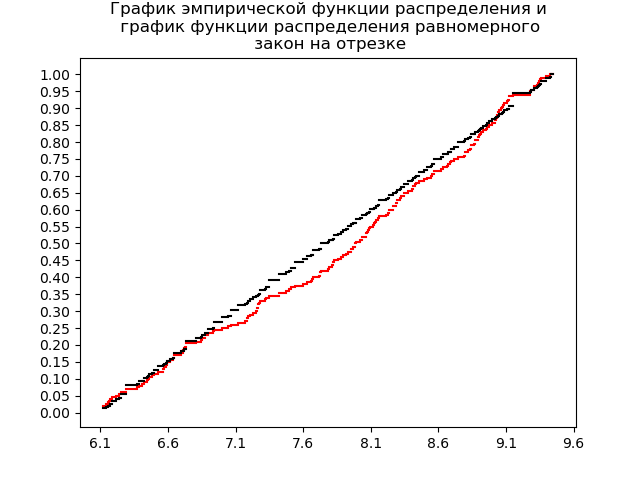
\includegraphics[width=1.0\textwidth]{../latex/inc/generated/img/EmpAndCurDistrFunc4.png}%
\end{figure}

%
$k_a=1.36000 \quad D_N \cdot \sqrt{N}=1.29855$

%
$1.29855 \le 1.36000$%
, то гипотеза о соответствии выборки показательному распределению не противоречит экспериментальным данным при уровне значисоти $a=0,05$